%%%%%%%%%%%%%%%%%%%%%%%%%%%%%%%%%%%%%%%%%%%%%%%%%%%%%%%%%%%%%%%%%%%%%%%%%%%%%%%%%%%%%%%%
%%
%%  Última alteração em 08/2013 por Rafael Pasquini (WTDCC 2013)
%%
%%%%%%%%%%%%%%%%%%%%%%%%%%%%%%%%%%%%%%%%%%%%%%%%%%%%%%%%%%%%%%%%%%%%%%%%%%%%%%%%%%%%%%%%

\documentclass[11pt]{article}
\usepackage{sbc-template}
\usepackage{graphicx,url}
%\usepackage[dvips]{graphicx}
%\usepackage[pdftex]{color,graphicx}
\usepackage{multicol}
\usepackage{multirow}
\usepackage{verbatim}
\usepackage{array}
\usepackage{amssymb,amsmath}
\usepackage[brazilian]{babel}
\usepackage[utf8]{inputenc}
\usepackage[T1]{fontenc}
\usepackage{tabularx}
\usepackage{mathtools}
\usepackage[table,xcdraw]{xcolor}

\sloppy

\title{4$^o$ Trabalho de Inteligência Computacional - Colônia de formigas}

\author{Autor: Gustavo Rezende Silva,\\ Orientador:Gina Maira Barbosa
de Oliveira}


\address{Faculdade de Computação\\
 Universidade Federal do Uberlândia (UFU)\\
  Uberlândia -- MG -- Brasil
  \email{gustavorezendesilva@hotmail.com, gina@ufu.br}
}

\begin{document}

\maketitle


\begin{resumo}
Este trabalho tem como intuito desenvolver um algoritmo de colônia de formigas (ACO)
para resolver o problema do caixero viajante (PCV). Podendo ter como entrada um
conjunto de vertices com suas coordenas ou distância entre os nós especifícadas.
\end{resumo}

\begin{palavraschave}
inteligência coletiva, algoritmo de colônia de formigas, caixero viajante, inteligência computacional
\end{palavraschave}

\section{Introdução}
\label{sec:intro}

O algoritmo de colônia de formigas é baseado no comportamento real das formigas
quando em grupos. Individualmente estes insetos não apresentam muita inteligência,
porém quando reunidos são capazes de realizar várias tarefas.

A comunicação das formigas é baseada no uso de feromônios, que é depositado
ao longo do caminho que elas percorrem. Para decidir qual caminho percorrer
estes insetos seguem, de maneira probabilistica, os caminhos com mais feromônios.
O comportamento das mesmas pode ser observado na fig. \ref{fig:ants}.

\begin{figure}[h]
  \centering
  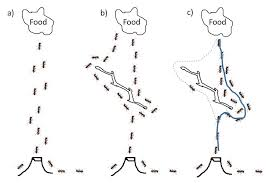
\includegraphics{ants.jpg}
  \caption{Comportamento das formigas no mundo real. Fonte: bioinfo3d.cs.tau.ac.il}
  \label{fig:ants}
\end{figure}

Um aspecto importante sobre os feromônios é que ele evapora com o tempo, ou seja,
quanto menos um caminho é percorrido menos chances ele tem de ser escolhido.

\section{Metodologia}
\label{sec:desen}

O algoritmo de colônia de formigas está respresentado de maneira simplificada na fig. \ref{fig:flux}.

\begin{figure}
  \centering
  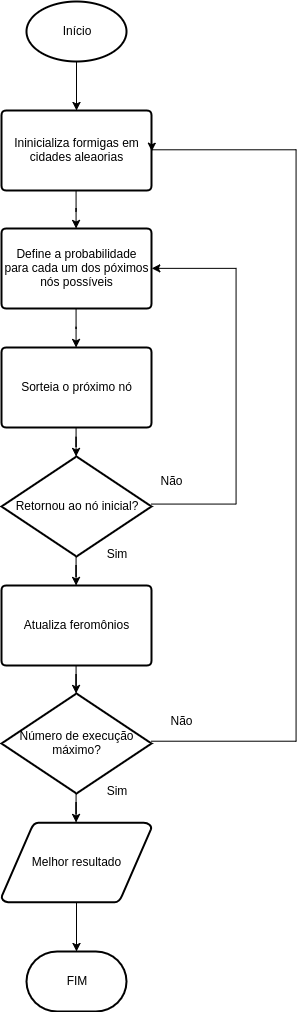
\includegraphics[height=10cm]{formigas.png}
  \caption{Fluxograma do algoritmo de colônia de formigas}
  \label{fig:flux}
\end{figure}

A primeira etapa para resolver o problema do caixero viajante utilizando o ACO é
colocar uma formiga em cada nó, ou distribui-las aleatóriamente. Cada um dos insetos
constroi uma solução individualmente.

Em seguida, a formiga escolhe para qual cidade irá se locomover probabilisticamente
seguindo a equação de probabilidade \ref{eq:prob}.

\begin{equation}\label{eq:prob}
  p_{ij}^{k}(t)=
  % \being{cases}
    \frac{(\tau_{ij}(t))^\alpha * (\eta_{ij})^\beta}{\sum_{l\in N_{i}^{k}}{(\tau_{ij}(t))^\alpha * (\eta_{ij})^\beta}}
  % \end{cases}
\end{equation}
Se j pertencer ao conjunto de soluções, caso contrario a probabilidade é igual a 0.

Onde:

$\tau_{ij}(t)$: quantidade de feromônio presente no caminho $(i,j)$

$\eta_{ij} = \frac{1}{d_{ij}}$: visibilidade da cidade $j$ com relação a cidade $i$

$\alpha$ e $\beta$ são parâmetros para determinar a influência do feromônio e da informação
heurística

$N_{i}{k}$ é a vizinhança factível da formiga $k$ (i.e., o conjunto
das cidades ainda não visitadas pela formiga $k$)

Ao ir para a próxima cidade a cidade anterior é retirada do conjunto de próximas
cidades permitidas. Então este processo é repetído até que a formiga passe por todas
as cidades, e depois ela retorna para a cidade inicial fechando o ciclo.

Após todas os nós terem sido visitados e a formiga retornado para a sua cidade inicial
os feromônios de cada aresta devem ser atualizados. Se a aresta $(i,j)$ pertence
a rota da formiga o depóstio de fernomônio nesta é calculado segundo a eq. \ref{eq:deltaf},
caso não esteja no caminho nada é adicionado.

E ainda, além do acréscimo de feromônio existe uma taxa de evaporação que é responsável
por retirar feromônio de todas as arestas a cada ciclo. A função completa para
atualizar o feromônio está demonstrada na eq. \ref{eq:fer}.

\begin{equation}\label{eq:deltaf}
  \Delta \tau_{ij}^{k} = \frac{Q}{L_{k}}
\end{equation}

 $Q$: quantidade de feromônio excretada por uma formiga a cada iteração

\begin{equation}\label{eq:fer}
  \tau_{ij}(t+1) = (1- \rho)\tau_{ij}(t) + \sum_{k=1}^{m}\Delta \tau_{ij}^{k}(t)
\end{equation}

 $\rho \in [0,1]$ é a taxa de evaporação de feronmônio

\section{Resultados}
\begin{table}[]
  \centering
  \caption{Tabela com resultados}
  \label{tab:resultados}
  \begin{tabular}{llllllll}
  \rowcolor[HTML]{000000}
  {\color[HTML]{FFFFFF} Problema} & {\color[HTML]{FFFFFF} Gerações} & {\color[HTML]{FFFFFF} alpha} & {\color[HTML]{FFFFFF} beta} & {\color[HTML]{FFFFFF} p} & {\color[HTML]{FFFFFF} Q} & {\color[HTML]{FFFFFF} Tempo{[}s{]}} & {\color[HTML]{FFFFFF} Resultado} \\
  M6                              & 50                              & 1                            & 2                           & 0.5                      & 1                        & 0,031                               & 2011                             \\
  M15                             & 50                              & 1                            & 2                           & 0.5                      & 1                        & 0,305                               & 7453                             \\
  M29                             & 50                              & 1                            & 2                           & 0.5                      & 1                        & 1,998                               & 28240                            \\
  M38                             & 50                              & 1                            & 2                           & 0.5                      & 1                        & 4,348                               & 6642
  \end{tabular}
\end{table}

\nocite{*}
\bibliographystyle{sbc}
\bibliography{bib}

\end{document}
